\chapter{Organisation et gestion de données}
{https://sacado.xyz/qcm/parcours_show_course/0/117141}
{
\begin{CpsCol}
{\LARGE \textbf{\color{sacado_violet}{Les savoir faire ciblés}}}
 \begin{itemize}[leftmargin=*]
 \item Savoir lire et compléter des données dans un tableau.
 \item Savoir lire et construire un diagramme en bâtons.
 \item Savoir utiliser et construire un diagramme circulaire.
 \item Savoir utiliser et construire un diagramme cartésien.
 \end{itemize}
\end{CpsCol}


\begin{CCon}
{\LARGE \textbf{\color{sacado_violet}{Chapitres connexes spiralés}}}
\begin{itemize}[leftmargin=*]
\item Proportionnalité
\item Angles
\end{itemize}
\end{CCon}

}
 
\begin{pageCours} 

\section{Tableaux}

\begin{DefT}{Tableau simple}

Les \textbf{tableaux}\index{Tableau} permettent d'organiser et de regrouper des données pour les lire plus facilement.
\begin{itemize}[leftmargin=*]
\item On utilise un tableau à \textbf{une seule entrée}\index{Simple|Tableau} pour organiser des données selon \textbf{un seul critère}.
\item On utilise un tableau à \textbf{double entrée}\index{A double entrée|Tableau} pour organiser des données selon \textbf{deux critères}, l'un qui est lu en ligne et l'autre en colonne.
\end{itemize}

\end{DefT}


\begin{ExT}{Tableau simple}

On a mesuré la taille d'une pousse de bambou lors des 6 premiers mois après sa plantation.
 \begin{center}
 \begin{tabular}{|c|c|c|c|c|c|c|} 
  \hline
  Mois & Novembre & Décembre & Janvier  & Février & Mars & Avril \\
  \hline
  Taille (cm) & \textcolor{sacado_green}{$70$} & $100$ & $127$ & \textcolor{sacado_violet}{$150$} & $180$ & \textcolor{sacado_orange}{$212$}  \\
  \hline
 \end{tabular}
 \end{center}

La pousse de bambou mesurent \textcolor{sacado_green}{$70$} cm lors de sa plantation en novembre. Au mois de février, elle mesure \textcolor{sacado_violet}{$150$} cm et \textcolor{sacado_orange}{$212$} cm en avril .
\end{ExT}


\begin{ExT}{Tableau à double entrée}

	Voici les résultats d'une enquête réalisée dans un collège sur le moyen de locomotion des élèves.

 \begin{center}
 \begin{tabular}{|c|c|c|c|c|c|c|} \hline
  Locomotion & A pied & Voiture & Bus &  Vélo & Autres & Total \\  \hline
  Garçons & $92$ & $36$ & \textcolor{sacado_orange}{$118$}& $54$ & $25$ & \textcolor{sacado_blue}{$325$} \\\hline
  Filles &  $94$ & $40$ & $197$ & \textcolor{sacado_violet}{$40$}  & $33$ & \textcolor{sacado_green}{$404$} \\\hline
  Total & \textcolor{sacado_gray}{$186$} & $76$ & $315$& \textcolor{sacado_red}{$94$} & $58$ & $729$ \\ \hline
 \end{tabular}
 \end{center}
 
\begin{itemize} 
 \item Dans ce collège, il y a \textcolor{sacado_green}{$404$} filles et \textcolor{sacado_blue}{$325$} garçons.
 \item \textcolor{sacado_gray}{$186$} élèves viennent à pied et \textcolor{sacado_red}{$94$} en vélo.
 \item \textcolor{sacado_violet}{$40$} filles viennent en vélo et \textcolor{sacado_orange}{$118$} garçons viennent en bus.
\end{itemize}

\end{ExT}

\end{pageCours}




\begin{pageAD} 

\Sf{Savoir lire des données dans un tableau à double entrée}

\ExoCad{Chercher. Communiquer. }

Voici les résultats d'une enquête réalisée dans un collège.

 \begin{center}
 \begin{tabular}{|c|c|c|c|}\hline 
  & Demi-pensionnaires & Externes & Total \\\hline 
  Garçons & $145$ & $173$ & $318$ \\\hline
  Filles & $70$ & $289$ & $359$ \\\hline
  Total & $215$ & $462$ & $677$ \\\hline 
 \end{tabular}
 \end{center}
 
 \begin{enumerate}[leftmargin=*]
 \item Quelles sont les deux entrées de ce tableau ? \point{2}
 \item Combien y a-t-il de garçons ? \point{1}
 \item Combien y a-t-il d'élèves externes ? \point{1}
 \item Combien d'élèves sont des filles demi-pensionnaires ? \point{1} 
 \item Que représente $173$ ? \point{1} 
\end{enumerate}

\Sf{Savoir compléter un tableau}

\ExoCad{Représenter.}

Le centre météorologique a enregistré les températures moyenne sur les 4 premiers mois de l'année : 15°C en avril, 7°C en janvier, 12°C en mars et 9°C en février. Complète le tableau suivant.

 \begin{center}
 \begin{tabular}{|c|c|c|c|c|}\hline 
  Mois & Janvier & Février & Mars & Avril \\\hline 
  Température ($\ldots$)& $\ldots$ & $\ldots$ & $\ldots$ & $\ldots$ \\\hline
 \end{tabular}
 \end{center}


\ExoCad{Représenter.}

Au championnat du monde de judo 2023, le japon a obtenu 5 médailles d'or, 2 d'argent et 4 de bronze. La France a glané 2 médailles d'or, 3 d'argent et 2 de bronze. Complète le tableau suivant.

 \begin{center}
 \begin{tabular}{|c|c|c|c|c|}\hline 
  Pays $\setminus$ médailles& Or & Argent & Bronze & Total\\\hline 
  Japon & $\ldots$ & $\ldots$ & $\ldots$ & $\ldots$ \\\hline
  France & $\ldots$ & $\ldots$ & $\ldots$& $\ldots$  \\\hline
 \end{tabular}
 \end{center}


\end{pageAD} 


\begin{pageCours} 
 
 
\section{Diagrammes en bâtons}

\begin{DefT}{Diagramme en bâtons}

Un \textbf{diagramme en bâtons}\index{diagramme en bâtons|Diagramme} est un \textbf{graphique} où les effectifs des données représentés par des \textbf{segments} dont les \textbf{hauteurs} sont \textbf{proportionnelles} à l'\textbf{effectif} de chaque donnée.
\end{DefT}

\begin{Ex}

Voici la liste des bateaux lors d'une course selon leur longueur.
\begin{center}

\begin{tabular}{|c|c|c|c|c|c|c|}\hline
Longueur (m) & $10$ & $11$ & $12$ & $13$ & $14$ & $15$ \\\hline
Effectif & $14$ & $3$ & $16$ & $3$ & $10$ & $5$ \\\hline
\end{tabular}

\begin{tikzpicture}
\begin{axis}[ybar,
grid=major,
ylabel=Effectif,
xlabel=Longueur (m),
x tick label style={/pgf/number format/1000 sep=}, 
xmin=10, 
xmax=15,
xtick distance=1,
ymin=0,
ymax=18,
enlarge x limits=0.15,
legend style={at={(.80,.95)},
anchor=north,legend columns=-1},
nodes near coords]
\addplot [draw=black,
%pattern=horizontal lines dark blue,
fill=sacado_violet,
] coordinates {
(10,14) (11,3) (12,16) (13,3) (14,10) (15,5)
};
\end{axis}

\end{tikzpicture}
\end{center}
\end{Ex}

\begin{Mt} 

Pour construire un diagramme à bâtons, on doit chercher les valeurs  extrêmes sur chaque ligne donnée. Ces  valeurs  extrêmes sont appelées \textbf{minimum}\index{minimum} et \textbf{maximum}\index{maximum}. La taille du graphique dépend de ces valeurs.

\end{Mt}

\end{pageCours}

\begin{pageAD} 

\Sf{Savoir lire un diagramme à bâtons}

\ExoCad{Représenter.}

Une école compte le nombre d'absences sur une semaine de 4 jours et consigne les données sur le graphique suivant.

\begin{minipage}{0.4\linewidth}

\begin{tikzpicture} 
\begin{axis}[
width=0.98\linewidth,ybar,
ylabel=Absence,
xlabel=Jour,
symbolic x coords={Lun.,Mar.,Jeu.,Ven.},
ymin=0,
ymax=13,
enlarge x limits=0.15,
legend style={at={(.80,.5)},
anchor=north,legend columns=-1},
nodes near coords]
\addplot [draw=black,
%pattern=horizontal lines,
fill=sacado_violet,
] coordinates {
(Lun.,11) (Mar.,8) (Jeu.,7) (Ven.,10)  
};
\end{axis}
\end{tikzpicture}

\end{minipage}
\begin{minipage}{0.6\linewidth}

\begin{enumerate}[leftmargin=*]
\item Combien d'absents sont-ils comptés le mardi ? \point{1}
\item Quel jour de la semaine compte-t-on $7$ absents ?  \point{1}
\item Quels jours de la semaine compte-t-on moins de $9$ absents ?  \point{1}
\end{enumerate}
\end{minipage}


\Sf{Savoir construire un diagramme à bâtons}

\ExoCad{Représenter.}

Le centre météorologique a enregistré les hauteurs de pluie sur les 4 premiers mois de l'année.

 \begin{center}
 \begin{tabular}{|c|c|c|c|c|}\hline 
  Mois & Janvier & Février & Mars & Avril \\\hline 
  Pluie (mm)& $15$ & $18$ & $9$ & $12$ \\\hline
 \end{tabular}
 \end{center}

Construis un diagramme à bâtons qui illustre cette étude.

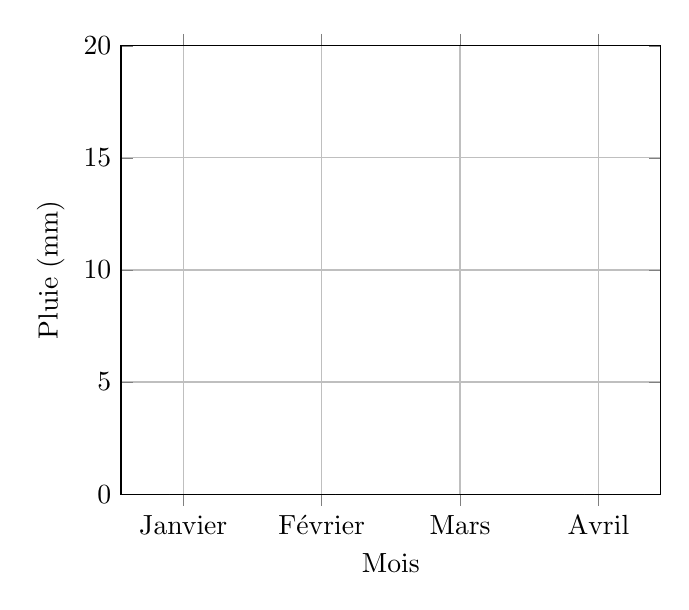
\begin{tikzpicture}
\begin{axis}[
grid=major,
%width=.98\linewidth,
ybar,
ylabel=Pluie (mm),
xlabel=Mois,
symbolic x coords={Janvier, Février, Mars, Avril},
ymin=0,
ymax=20,
enlarge x limits=0.15,
]
\addplot [draw=black,
fill=white!0,
] coordinates {
(Janvier,0) (Février,0) (Mars,0) (Avril,0)
};
\end{axis}
\end{tikzpicture}


\end{pageAD}



\begin{pageCours} 

\section{Diagrammes circulaires}
\begin{DefT}{diagramme circulaire}

Un \textbf{diagramme circulaire}\index{diagramme circulaire|Diagramme} est un \textbf{graphique} où les effectifs des données sont représentés par des \textbf{secteurs angulaires} dont les \textbf{mesures des angles} sont \textbf{proportionnelles} à l'\textbf{effectif} de chaque donnée. 

\end{DefT}

\begin{Ex}

Dans une recette de cuisine, on lit les ingrédients :

$140\,g$ de farine, $190\,g$ de sucre, $150\,g$ de chocolat et $260\,g$ de beurre.

\begin{minipage}{0.48\linewidth}

\begin{tabular}{|c|c|c|}\hline
Nom & Donnée ($g$) & Angle (°) \\\hline
Farine &  \textcolor{sacado_violet}{$140$} & $68,1$ \\\hline
Sucre & \textcolor{bleu2}{$190$} & $92,4$ \\\hline
Chocolat &  \textcolor{sacado_yellow}{$150$} &  $73$ \\\hline
Beurre & \textcolor{sacado_orange}{$260$} & $126,5$ \\\hline
Total & $740$ &  $360$ \\\hline
\end{tabular}
\end{minipage}
\begin{minipage}{0.48\linewidth}
\begin{tikzpicture}
\pie[pos={0,0}, sum=auto,radius=1.25,text=pin]{260/Beurre,  140/Farine, 150/Chocolat, 190/Sucre};
\end{tikzpicture}
\end{minipage}

\end{Ex}


\begin{Mt}

\begin{enumerate}[leftmargin=*]
\item Pour construire un diagramme circulaire, il faut convertir chaque donnée en une mesure d'angle.
\item Construire un cercle de rayon assez grand, on peut imaginer $5$ cm.
\item Tracer les angles obtenus à la phase \textbf{1}. 
\end{enumerate}
 
\end{Mt}


\end{pageCours}


\begin{pageAD} 

\Sf{Lire un diagramme circulaire }

\ExoCad{Chercher.}

Voici le diagramme circulaire des dépenses d'un club de foot, exprimés en Millions d'euros.

\begin{minipage}{0.58\linewidth}

\begin{tikzpicture}
\pie[pos={0,0}, sum=auto,radius=2,text=pin]{300/Salaires, 190/Matériels, 150/Infrastructure,50/Publicité, 20/Voyages};
\end{tikzpicture}

\end{minipage} 
\begin{minipage}{0.38\linewidth}
\begin{enumerate}[leftmargin=*]
\item Quelle est la somme totale des dépenses ? \point{3}
\item Quelle est la dépense liée à la publicité ? \point{1}
\item Quelle est la part salariale du club ? \point{3}
\end{enumerate}
\end{minipage}

\Sf{Construire un diagramme circulaire }

\ExoCad{Représenter. Calculer.}

Dans un collège, on compte $243$ externes,  $123$ demi-pensionnaires et $32$ internes.

\begin{enumerate}
\item Complète le tableau.

\begin{tabular}{|c|c|c|}\hline
Statut & Données & Angle (°) \\\hline
Externes &  $\ldots$  & $\ldots\ldots$ \\\hline
Demi-pensionnaires & $\ldots$ & $\ldots\ldots$  \\\hline
Internes & $\ldots$  & $\ldots\ldots$  \\\hline
Total &  $\ldots$ &  $360$ \\\hline
\end{tabular}

\item Trace un cercle de rayon $5$ cm et construis chaque secteur angulaire avec  la bonne légende.
\end{enumerate}


\end{pageAD}


\begin{pageCours}

\section{Diagrammes cartésiens}

\begin{DefT}{Axe des abscisses. Axe des ordonnées }
Pour \textbf{représenter} une grandeur B \textbf{en fonction d'}une grandeur A, on place :
\begin{itemize}[leftmargin=*]
\item Sur l'\textbf{axe horizontal} (appelé  \textbf{axe des abscisses} )\index{Axe des abscisses} les valeurs de la grandeur A.
\item Sur l'\textbf{axe vertical} (appelé  \textbf{axe des ordonnées} )\index{Axe des ordonnées} les valeurs de la grandeur B.
\end{itemize}
\end{DefT}

\begin{Ex}
On a relevé la température pendant une journée à Bogotá (Colombie).
\begin{center}
\begin{tabular}{|c|c|c|c|c|c|c|c|c|c|c|c|c|}
\hline
Heure & $0$ & $2$ & $4$ & $6$ & $8$ & $10$ & $12$ & $14$ & $16$ & $18$ & $20$ & $22$ \\
\hline
Temp (°C) & $6$ & \cellcolor{blue!20}$5$ & $4$  & \cellcolor{orange!20}$8$ & $11$ & $14$ &  \cellcolor{magenta!20}$18$ &  \cellcolor{yellow!20}$15$ & $13$ &  \cellcolor{green!20}$10$ & $8$ & $7$ \\
\hline
\end{tabular}

 
\vspace{.2cm}

\begin{tikzpicture}
  \begin{axis}[
  	grid=major,
    xlabel={Heures},
    ylabel={Temperature (°C)},
    %symbolic x coords={Jan,Fev,Mar,Avr,Mai,Jun,Jul,Agu,Sep,Oct,Nov,Dec},
	ytick={0,2,4,6,8,10,12,14,16,18,20,22},
	ymin=0,
	xmin=0,
	xtick={0,2,4,6,8,10,12,14,16,18,20,22},
    width=\linewidth,
    height=8cm,
  ]
  \addplot[mark=+, mark options={draw=blue, fill=blue},mark size=4pt] coordinates {
    (2, 5)
  };
  
  \addplot[mark=+, mark options={draw=orange, fill=orange},mark size=4pt] coordinates {
    (6, 8)
  };
  \addplot[mark=+, mark options={draw=magenta, fill=magenta},mark size=4pt] coordinates {
    (12, 18)
  };
  \addplot[mark=x, mark options={draw=yellow, fill=yellow},mark size=4pt] coordinates {
    (14, 15)
  };
  \addplot[mark=+, mark options={draw=green, fill=green},mark size=4pt] coordinates {
    (18, 10)
  };
  \addplot [sacado_violet] coordinates {
(0,6) (2,5) (4,4) (6,8) (8,11) (10,14) (12,18) (14,15) (16,13) (18,10) (20,8) (22,7)
};
  
  \end{axis}
\end{tikzpicture}
\end{center}
\begin{itemize}
\item A $2$h, la température est de $5$°C et à $6$h, la température est de $8$°C.
\item Il fait le plus chaud à midi avec une température de $18$°C.
\item La température la plus froide est $4$°C à 4h du matin. 
\item De $6$h à $20$h, la température est supérieure à $8$°C.  
\end{itemize}
\end{Ex}

\end{pageCours}




\begin{pageAD}

\Sf{Lire un diagramme cartésien }

\ExoCad{Chercher.}

\begin{minipage}{0.58\linewidth}

Voici le graphique des précipitations durant $24$ heures.
 
\begin{tikzpicture}
  \begin{axis}[
  	grid=major,
    xlabel={Heures},
    ylabel={Précipitations (mm)},
    %symbolic x coords={Jan,Fev,Mar,Avr,Mai,Jun,Jul,Agu,Sep,Oct,Nov,Dec},
	ytick={0,1,2,3,4,5,6,7,8,9,10,11,12,13,14,15,16,17,18,19,20},
	ymin=0,
	xmin=0,
	xtick={0,2,4,6,8,10,12,14,16,18,20,22},
    width=\linewidth,
    height=8cm,
  ]
  \addplot [sacado_violet] coordinates {
(0,10) (2,15) (4,14) (6,8) (8,3) (10,0) (12,0) (14,0) (16,3) (18,5) (20,8) (22,3)
};
  
  \end{axis}
\end{tikzpicture}

\end{minipage} 
\begin{minipage}{0.38\linewidth}

\begin{enumerate}[leftmargin=*]
\item Quelle est la hauteur des précipitations à 6h ? \point{1}
\item Quelle est la hauteur des précipitations à 12h ? \point{1}
\item Quelle est la hauteur des précipitations à 20h ? \point{1}
\item A quelle heure les précipitations sont-elles les plus abondantes ? \point{1}
\item A quelle heure la pluie s'est-elle arrêtée ?  \point{1}
\end{enumerate}


\end{minipage} 



\Sf{Construire un diagramme cartésien }

\ExoCad{Représenter. Calculer.}

Les parents de Laure ont mesuré sa taille pendant sa première année.
\begin{center}
\begin{tabular}{|c|c|c|c|c|c|c|c|c|c|c|c|c|}\hline
Mois & $0$ & $1$ & $2$ & $3$ & $4$ & $5$ & $6$ & $7$ & $8$ & $9$ & $10$ & $11$ \\\hline
Taille (cm) & $48$ & $50$ & $53$ & $56$ & $60$ & $62$ & $64$ & $66$ & $68$ &$70$ & $72$ & $74$ \\\hline
\end{tabular}
\end{center}

Construis le diagramme cartésien de cette situation.

\begin{center}

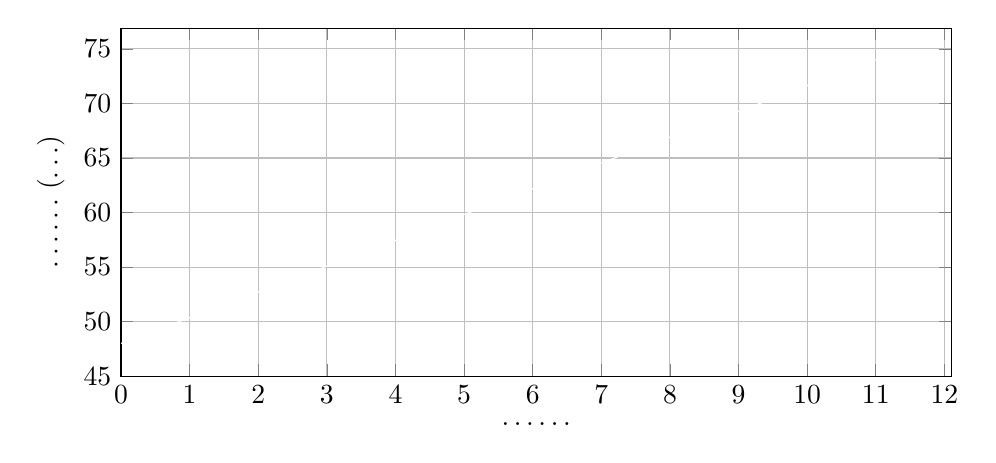
\begin{tikzpicture}
  \begin{axis}[
  	grid=major,
    xlabel={$\ldots\ldots$},
    ylabel={$\ldots\ldots$ ($\ldots$)},
    %symbolic x coords={Jan,Fev,Mar,Avr,Mai,Jun,Jul,Agu,Sep,Oct,Nov,Dec},
	ytick={45,50,55,60,65,70,75},
	ymin=45,
	xmin=0,
	xtick={0,1,2,3,4,5,6,7,8,9,10,11,12},
    width=\linewidth,
    height=6cm,
  ]
  
   \addplot [white!0] coordinates {
(0,48)  (11,74)
}; 
  
  \end{axis}
\end{tikzpicture}

\end{center}


\end{pageAD}



%%%%%%%%%%%%%%%%%%%%%%%%%%%%%%%%%%%%%%%%%%%%%%%%%%%%%%%%%%%%%%%%%%%
%%%  Niveau 1
%%%%%%%%%%%%%%%%%%%%%%%%%%%%%%%%%%%%%%%%%%%%%%%%%%%%%%%%%%%%%%%%%%
\begin{pageParcoursu} 

\ExoCu{Chercher. Communiquer.}

Le golf se joue en un minimum de coup. Pour chaque trou, le golfeur doit respecter un contrat, appelé "\textbf{par}", nombre de coups à jouer. On a représenté le par des 9 premiers trous du parcours. 

 \begin{center}
 \begin{tabular}{|c|c|c|c|c|c|c|c|c|c|} \hline
  Trou  & $1$ & $2$ & $3$ &  $4$ & $5$ & $6$  &  $7$ & $8$ & $9$ \\  \hline
  Par & $4$ & $4$ &$3$ & $5$ & $4$ &  $3$ & $4$ &$4$ & $5$   \\\hline
 \end{tabular}
 \end{center}
 
\begin{enumerate}[leftmargin=*] 
 \item Quel est le par du trou $6$ ? \point{1}
 \item Combien y a-t-il de par $5$ ? \point{1}
 \item Quel est le par des $9$ premiers trous ? \point{1}
\end{enumerate} 
 


\ExoCu{Chercher. Communiquer.}

Un randonneur parcours 4 km et reporte sa vitesse de marche sur le graphique.

\begin{minipage}{0.38\linewidth}
\begin{center}
\begin{tikzpicture}
  \begin{axis}[
  	grid=major,
    xlabel={Distance (km)},
    ylabel={Vitesse (km/h)},
	ytick={0,1,2,3,4,5,6},
	ymin=0,
	ymax=7,
	xmin=0,
	xtick={0,1,2,3,4},
    width=\linewidth,
    height=4cm,
  ]

  \addplot [sacado_violet] coordinates {
(0,0)(0.1,6)  (1,3) (2,4) (3,3) (4,6)
}; 
  \end{axis}
\end{tikzpicture}
\end{center}
\end{minipage}
\begin{minipage}{0.58\linewidth}
 \begin{enumerate}
 	\item Quelle est la vitesse au 2ème km ? \point{1}
 	\item Quelle est la vitesse maximale ? \point{1}
 	\item Est-il vrai que la vitesse est tombée à $1$ km/h ?\point{2}
 \end{enumerate}
\end{minipage} 
 
 
\ExoCu{Chercher. Communiquer.}


Dans une auberge de jeunesse, il y a  200 voyageurs dont des français, des espagnols, des italiens et des belges. Le diagramme suivant représente chaque nationalité


\begin{minipage}{0.48\linewidth}
\definecolor{ffdxqq}{rgb}{1.,0.8431372549019608,0.}
\definecolor{ffqqqq}{rgb}{1.,0.,0.}
\definecolor{qqwuqq}{rgb}{0.,0.39215686274509803,0.}
\definecolor{qqqqff}{rgb}{0.,0.,1.}
\definecolor{xdxdff}{rgb}{0.49019607843137253,0.49019607843137253,1.}
\definecolor{uuuuuu}{rgb}{0.26666666666666666,0.26666666666666666,0.26666666666666666}
\begin{tikzpicture}[line cap=round,line join=round,>=triangle 45,x=1.0cm,y=1.0cm]
\clip(-3.3,-3.14) rectangle (3.7,3.32);
\fill[line width=2.pt,color=ffdxqq,fill=ffdxqq,fill opacity=0.6] (0.,0.) -- (1.9881505889355497,-2.246610165497171) -- (3.,0.) -- cycle;
\fill[line width=2.pt,color=ffqqqq,fill=ffqqqq,fill opacity=0.6] (0.,0.) -- (-1.0077573305663405,-2.8256725151173843) -- (1.9881505889355497,-2.246610165497171) -- cycle;
\fill[line width=2.pt,color=qqwuqq,fill=qqwuqq,fill opacity=0.6] (0.,3.) -- (0.,0.) -- (-1.0077573305663405,-2.8256725151173843) -- cycle;
\fill[line width=2.pt,color=qqqqff,fill=qqqqff,fill opacity=0.6] (0.,0.) -- (0.,3.) -- (3.,0.) -- cycle;
\draw [line width=2.pt] (0.,0.) circle (3.cm);
\draw [shift={(0.,0.)},line width=2.pt,color=qqqqff,fill=qqqqff,fill opacity=0.6]  plot[domain=0.:1.5707963267948966,variable=\t]({1.*3.*cos(\t r)+0.*3.*sin(\t r)},{0.*3.*cos(\t r)+1.*3.*sin(\t r)});
\draw [shift={(0.,0.)},line width=2.pt,color=qqwuqq,fill=qqwuqq,fill opacity=0.6]  plot[domain=1.5707963267948966:4.36980810595183,variable=\t]({1.*3.*cos(\t r)+0.*3.*sin(\t r)},{0.*3.*cos(\t r)+1.*3.*sin(\t r)});
\draw [shift={(0.,0.)},line width=2.pt,color=ffqqqq,fill=ffqqqq,fill opacity=0.6]  plot[domain=4.36980810595183:5.436829893692564,variable=\t]({1.*3.*cos(\t r)+0.*3.*sin(\t r)},{0.*3.*cos(\t r)+1.*3.*sin(\t r)});
\draw [shift={(0.,0.)},line width=2.pt,color=ffdxqq,fill=ffdxqq,fill opacity=0.6]  plot[domain=-0.8463554134870224:0.,variable=\t]({1.*3.*cos(\t r)+0.*3.*sin(\t r)},{0.*3.*cos(\t r)+1.*3.*sin(\t r)});
\draw (-2.28,0.48) node[anchor=north west] {Espagnols};
\draw (1.,1.58) node[anchor=north west] {Français};
\draw (-0.2,-1.58) node[anchor=north west] {Italiens};
\draw (1.58,-0.64) node[anchor=north west] {Belges};
\end{tikzpicture}
\end{minipage}
\begin{minipage}{0.48\linewidth}
\begin{enumerate}[leftmargin=*]
\item Quelle est la nationalité la plus représentée ?\point{1}
\item Quelle est le nombre de français ? \point{1}
\item Classe les nationalités par ordre croissant du nombre de ressortissants.\point{2}
\item Est-il vrai que les espagnols sont deux fois plus nombreux que les français ?\point{2}
\end{enumerate}
\end{minipage}


 
 
\end{pageParcoursu}


%%%%%%%%%%%%%%%%%%%%%%%%%%%%%%%%%%%%%%%%%%%%%%%%%%%%%%%%%%%%%%%%%%%
%%%%  Niveau 2
%%%%%%%%%%%%%%%%%%%%%%%%%%%%%%%%%%%%%%%%%%%%%%%%%%%%%%%%%%%%%%%%%%%
\begin{pageParcoursd} 

\ExoCd{Représenter. Calculer.} 

 Voici les données de précipitations (en $mm$) sur la ville de Tunis au cours de l'année 2021 : 
\begin{center}
\begin{tabular}{|c|c|c|c|c|c|c|c|c|c|c|c|c|}\hline
Mois & J & F & M & A & M & J & J & A & S & O & N & D \\\hline
Précipitations (en $mm$) & 56 & 53 & 48 & 43 & 27 & 11 & 2 & 9 & 38 & 51 & 52 & 54 \\\hline
\end{tabular}
 \end{center}

Représenter ces données à l'aide d'un diagramme à bâtons.
 
\begin{center}
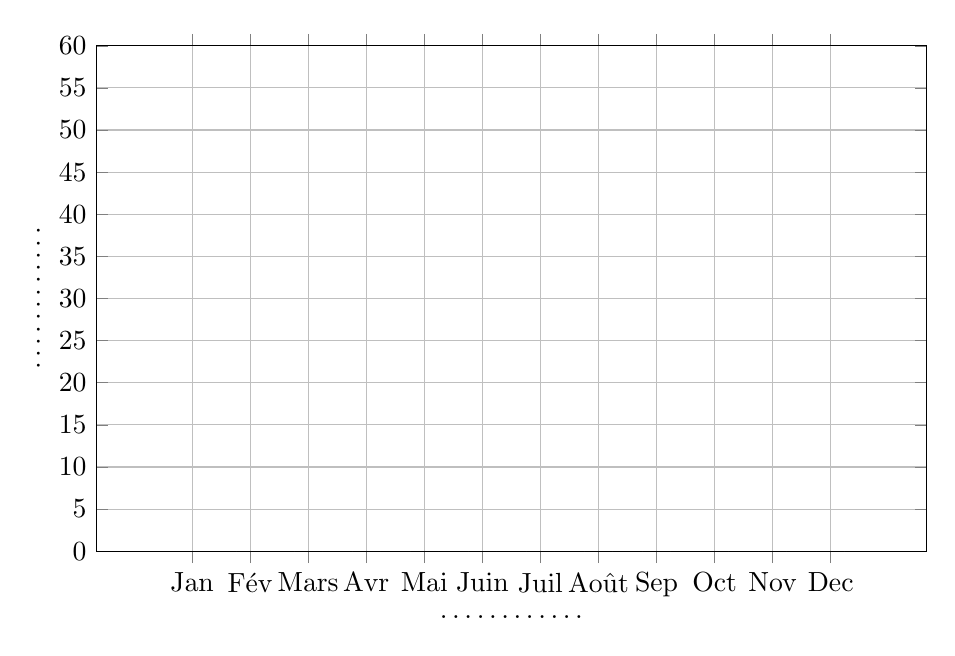
\begin{tikzpicture}
\begin{axis}[
grid=major,
width=.98\linewidth,
ybar,
ylabel=$\ldots\ldots\ldots\ldots$,
xlabel=$\ldots\ldots\ldots\ldots$,
symbolic x coords={Jan, Fév, Mars, Avr, Mai, Juin, Juil, Août, Sep, Oct, Nov, Dec},
xtick={Jan, Fév, Mars, Avr, Mai, Juin, Juil, Août, Sep, Oct, Nov, Dec},
ytick={0, 5, 10, 15, 20, 25, 30, 35, 40, 45, 50, 55, 60},
ymin=0,
ymax=60,
enlarge x limits=0.15,    
width=\linewidth,
height=8.0cm,
]
\addplot [draw=black,
fill=white!0,
] coordinates {
(Jan,0) (Fév,0) (Mars,0) (Avr,0)(Mai,0) (Juin,0) (Juil,0) (Août,0)(Sep,0) (Oct,0) (Nov,0) (Dec,0)
};
\end{axis}
\end{tikzpicture}
\end{center}
 
 
 \ExoCd{Représenter. Calculer. Communiquer.}
 
 
Dans un collège il y a $328$ filles et $326$ garçons. $190$ garçons sont externes et $140$ filles sont demi-pensionnaires.

\begin{enumerate}[leftmargin=*]
 \item Complète le tableau avec les données.
 \begin{center}
 \begin{tabular}{|c|c|c|c|} \hline
    & Externes & Demi-pensionnaire &  Total \\  \hline
  Filles &    &   & \\\hline
  Garçons &  &   &  \\\hline
  Total & &  & \\ \hline
 \end{tabular}
 \end{center}
 
 \item Quel est le nombre d'externes ? \point{1} 
 \item Combien de garçons sont demi-pensionnaires ? \point{1} 
 \item Combien de filles sont externes ? \point{1}
\end{enumerate}


\end{pageParcoursd}

%%%%%%%%%%%%%%%%%%%%%%%%%%%%%%%%%%%%%%%%%%%%%%%%%%%%%%%%%%%%%%%%%%%
%%%%  Niveau 3
%%%%%%%%%%%%%%%%%%%%%%%%%%%%%%%%%%%%%%%%%%%%%%%%%%%%%%%%%%%%%%%%%%%
\begin{pageParcourst}

\ExoCt{Représenter.}
 
Un institut de recherche agronomique a mesuré les longueurs des feuilles de lauriers en fonction des jours.

 \begin{center}
 \begin{tabular}{|c|c|c|c|c|c|c|c|c|c|c|} \hline
  jour  & $1$ & $2$ & $3$ & $4$ & $5$ & $6$ & $7$ & $8$ & $9$ & $10$   \\  \hline
  longueur (mm) & $1$ & $4$ & $6$ & $8$ & $10$ & $13$& $14$ & $16$ &$19$ &$20$\\\hline
 \end{tabular}
 \end{center}
 
 Construis le diagramme cartésien des données :
 
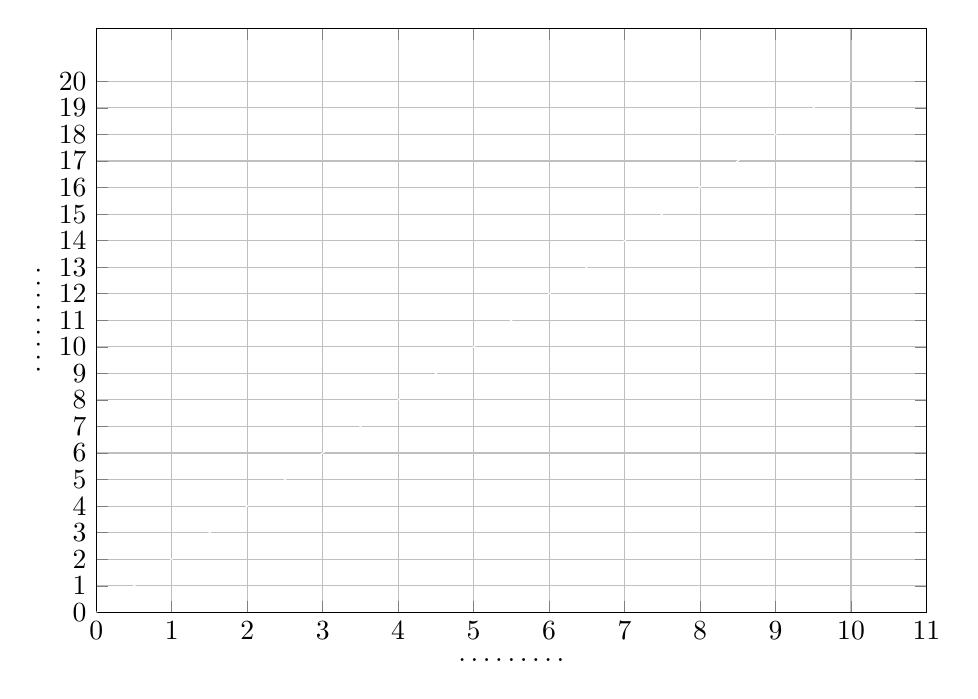
\begin{tikzpicture}
  \begin{axis}[
  	grid=major,
    xlabel={$\ldots\ldots\ldots$},
    ylabel={$\ldots\ldots\ldots$},
    %symbolic x coords={Jan,Fev,Mar,Avr,Mai,Jun,Jul,Agu,Sep,Oct,Nov,Dec},
	ytick={0,1,2,3,4,5,6,7,8,9,10,11,12,13,14,15,16,17,18,19,20},
	ymin=0,
	xmin=0,
	xtick={0,1,2,3,4,5,6,7,8,9,10,11,12,13,14,15,16,17,18,19,20},
    width=\linewidth,
    height=9cm,
  ]
 \addplot [draw=white!0,
fill=white!0,
] coordinates {
(0,0) (10,20)
};
  \end{axis}
\end{tikzpicture}
 
\ExoCt{Représenter. Calculer.}


 Construis un diagramme circulaire représentant la répartition des sources énergétiques en France en 2021.

 \begin{minipage}{0.6\linewidth}

\begin{center}
\begin{tabular}{|c|c|c|}\hline
\textbf{Source} & \textbf{2021} (en \%)& \textbf{2021} (en °)\\\hline
\textbf{Produits pétroliers} &	$28$ &$\ldots$ \\\hline
\textbf{Nucléaire} &	$40$ &$\ldots$ \\\hline
\textbf{Gaz naturel} &	$15$ &$\ldots$ \\\hline
\textbf{Charbon} &	$4$ &$\ldots$ \\\hline
\textbf{Energies renouvelables} &  $13$ & $\ldots$ \\\hline
\textbf{Total} &   $\ldots$ &$\ldots$  \\\hline
\end{tabular}
\end{center}
\end{minipage}
 \begin{minipage}{0.4\linewidth}
 

\begin{tikzpicture}[line cap=round,line join=round,>=triangle 45,x=1.0cm,y=1.0cm]
\clip(-3.24,-3.04) rectangle (3.3,3.12);
\draw [line width=2.pt] (0.,0.) circle (2.5cm);
\begin{scriptsize}
\draw [color=black] (0.,0.)-- ++(-2.0pt,0 pt) -- ++(4.0pt,0 pt) ++(-2.0pt,-2.0pt) -- ++(0 pt,4.0pt);
\end{scriptsize}
\end{tikzpicture}
 \end{minipage} 
 

\end{pageParcourst}

%%%%%%%%%%%%%%%%%%%%%%%%%%%%%%%%%%%%%%%%%%%%%%%%%%%%%%%%%%%%%%%%%%%
%%%%  Brouillon
%%%%%%%%%%%%%%%%%%%%%%%%%%%%%%%%%%%%%%%%%%%%%%%%%%%%%%%%%%%%%%%%%%%


\begin{pageBrouillon} 
 
\ligne{32}



\end{pageBrouillon}



\begin{pageAuto} 

 
\ExoAuto
 
Une compagnie aérienne ouvre une nouvelle ligne quotidienne et note le nombre de passagers par vol pendant deux semaines dans le tableau ci-dessous.

\begin{center}
\begin{tabular}{|c|c|c|c|c|c|c|c|c|}\hline 
 &  lundi	& mardi & mercredi& jeudi& vendredi& samedi& dimanche & total \\\hline
\textbf{Semaine $1$}  &  $186$	& $188$	 & $158$	& $158$	& $190$	& $182$	& $125$	 & $\ldots\ldots$	\\\hline
\textbf{Semaine $2$}  &  $172$  & $175$	 & $177$	& $154$	& $189$	& $180$	& $123$	 & $\ldots\ldots$\\\hline 
\textbf{Total}  &  $\ldots\ldots$  & $\ldots\ldots$	 & $\ldots\ldots$	& $\ldots\ldots$	& $\ldots\ldots$	& $\ldots\ldots$	& $\ldots\ldots$	 & $\ldots\ldots$\\\hline 
\end{tabular}
\end{center}

\begin{enumerate}
\item Complète le tableau.
\item Combien de voyageurs prennent-ils cette compagnie le jeudi de la semaine 1 ? $\ldots\ldots\ldots$
\item Combien de voyageurs prennent-ils cette compagnie le mercredi de la semaine 2 ? $\ldots\ldots$
\item Combien de voyageurs prennent-ils cette compagnie la semaine 2 ? $\ldots\ldots\ldots\ldots\ldots\ldots$
\item Quel est le jour de la première semaine où il y a le plus de voyageurs  ? $\ldots\ldots\ldots\ldots\ldots$
\item Quel est le jour sur ces deux semaines où il y a le moins de voyageurs  ? $\ldots\ldots\ldots\ldots\ldots$
\end{enumerate}

\ExoAuto

 \begin{minipage}{0.48\linewidth}
 Voici les données sur les différentes énergies en France. 
 
 \vspace{0.2cm}
 
 Représenter les données suivantes sous forme de diagrammes circulaires, un pour l'année 2019, un pour l'année 2020.
\end{minipage}
 \begin{minipage}{0.5\linewidth}
\begin{center}
\begin{tabular}{|c|c|c|}\hline 
\textbf{Source} & \textbf{2019} (en \%) & \textbf{2020} (en \%) \\\hline 
\textbf{Fossile} &	81,2 &	82,2\\\hline
\textbf{Hydraulique} &  1,2	& 1,1\\\hline
\textbf{Éolienne} & 4,6	& 4,4\\\hline
\textbf{Solaire} & 0,2 & 0,2\\\hline 
\end{tabular}
\end{center}
\end{minipage}


\begin{minipage}{0.48\linewidth}

\begin{center}

\begin{tikzpicture}[line cap=round,line join=round,>=triangle 45,x=1.0cm,y=1.0cm]
\clip(-3.24,-3.04) rectangle (3.3,3.12);
\draw [line width=2.pt] (0.,0.) circle (2.3cm);
\begin{scriptsize}
\draw [color=black] (0.,0.)-- ++(-2.0pt,0 pt) -- ++(4.0pt,0 pt) ++(-2.0pt,-2.0pt) -- ++(0 pt,4.0pt);
\end{scriptsize}
\end{tikzpicture}

\textbf{Année 2019}
\end{center}
\end{minipage}
\begin{minipage}{0.5\linewidth}
\begin{center}
\begin{tikzpicture}[line cap=round,line join=round,>=triangle 45,x=1.0cm,y=1.0cm]
\clip(-3.24,-3.04) rectangle (3.3,3.12);
\draw [line width=2.pt] (0.,0.) circle (2.3cm);
\begin{scriptsize}
\draw [color=black] (0.,0.)-- ++(-2.0pt,0 pt) -- ++(4.0pt,0 pt) ++(-2.0pt,-2.0pt) -- ++(0 pt,4.0pt);
\end{scriptsize}
\end{tikzpicture}

\textbf{Année 2020}
\end{center}
\end{minipage} 



\end{pageAuto}
